\chapter{MARCO TEORICO}

\section{Tecnologia de membranas}
\subsection{Aspectos generales de la separacion por membranas}

Existen muchas definiciones para una membrana, sin embargo, de forma general, se define como una barrera delgada, situada entre dos fases o medios, lo que permite el paso selectivo de uno o más constituyentes de un medio a otro, en presencia de una fuerza impulsora apropiada, mientras se retiene el resto \parencite[p.~3]{Pabby2015} 

% ------------ Comando para insercion de figuras ------------------
\begin{figure}[ht]
\caption{Esquema general de un sistema de membrana. Tomado de Drioli, et al. (2018) \textit{Membrane Engineering} (P.2) DE GRUYTER. Figura 1.2}
\centering
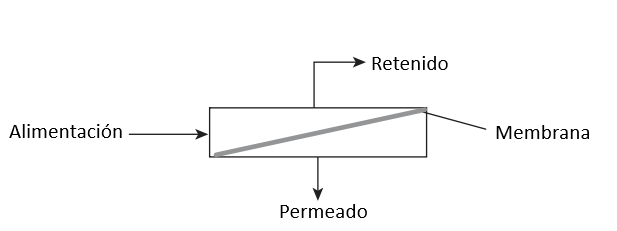
\includegraphics[width = 1\textwidth]{Figuras/esquema general de sistemas de membrana.png}
\label{fig:sep_membranas}
\end{figure}

De forma general, un sistema de membranas está conformado por cuatros componentes: una corriente de alimentación, una membrana, una corriente de permeado, que contiene las especies que han pasado a través de la membrana y una corriente de retenido o residuo (también denominado concentrado), que contiene especies que han sido excluidas o retenidas, y que no han pasado a través de la estructura de la membrana \parencite[p~8]{Singh2014}. La representación esquemática general de un sistema de membrana se muestra en la Figura \ref{fig:sep_membranas} con sus cuatro componentes.

La eficiencia de la separación en un sistema de membranas depende de algunas variables como el tipo de membrana, el modelo de difusión, fuerza impulsora, obstrucción en la membrana, etc., sin embargo, de forma general, la eficiencia de la separación puede ser cuantificada mediante el coeficiente de rechazo (R) que indica la habilidad de separación del proceso de membrana y se puede obtener mediante la Ecuación \ref{eq:RechazoMembrana} donde C1 representa la concentración del soluto en la alimentación del sistema y C2 representa la concentración del producto \parencite[p~13]{Singh2014} 

% ------------ Comando para insercion de ecuaciones ---------------
\begin{equation}
R = \frac{C_1 - C_2}{C_1} \times 100
\label{eq:RechazoMembrana}
\end{equation}

\subsection{Procesos de separación por membrana}
Los procesos de separación por membrana se pueden clasificar de manera general en función de su fuerza impulsora, ya sea debido a un gradiente de presión, temperatura, concentración, potencial eléctrico o vacío.

Los procesos impulsados por la presión se muestran en la Tabla \ref{tab:procesos de membrana}, donde las principales diferencias entre un proceso y otro son las presiones transmembrana con las que se operan para aumentar la velocidad del proceso de transporte y el rango de tamaño de partículas o solutos que son separados. Los procesos de Microfiltración (MF) se caracterizan por ser usualmente procesos de clarificación que separan las moléculas y partículas en base a su tamaño y solubilidad \parencite[p~7]{Nath2017}. Además, los procesos MF son los que tienen un menor requerimiento energético, en comparación con los demás procesos descritos en la Tabla \ref{tab:procesos de membrana}, debido a que las membranas utilizadas poseen mayores tamaños de poros, lo que permite que se puedan operar a menores presiones.

%-------------- Comando para tablas -------------------------

\begin{table}[ht]
\small    
\caption{Procesos de membrana impulsados por la presión}
    \centering
    \begin{tabular}{p{4cm} p{4cm} p{4cm} p{4cm}}
         \toprule
        Proceso de membrana & Presión transmembrana (bar) & Permeado & Retenido \\
         \midrule
        Microfiltración & 1 - 2 & Solutos disueltos, agua & Partículas retenidas, agua \\
        Ultrafiltración & 1 - 5 & Pequeñas moléculas, agua & Polímeros, proteínas, coloides particulados \\
        Nanofiltración & 5 - 15 & Iones monovalentes, agua & Pequeñas moléculas, sales divalentes \\
        Ósmosis inversa & 15 - 100 & Agua, pequeños solventes polares, sales & Todos los solutos, agua \\
         \bottomrule
    \end{tabular}
    \label{tab:procesos de membrana}
\end{table}
\small \textbf{Nota:} Traducido de Membrane Technology in Separation Science (P. 6) de M. Purkait, R. Singh (2008). CRC Press y Membrane separation Processes (P.7) de K. Nath (2017) PHI Learning Private Limited.
